\section{Análisis de arquitectura tolerante a fallas}
\begin{frame}
	\begin{block}{Se supone una misión:}
		\begin{itemize}
			\item Misión de 15 años. 
			\item Sin payload.
			\item Formados por 6 subsistemas. 
			\item Como mínimo se tomarán 6 nodos en representación de los subsistemas.
			\item Cada nodo es una computadora con capacidad de procesamiento. 
			\item Cada nodo es un componente COTS.
		\end{itemize}
	\end{block}
\end{frame}

\begin{frame}
	Se concluye que las topologías que cumplen con los requerimientos y los objetivos de este trabajo de tesis son:
	\begin{itemize}
		\item Árboles binarios
		\item Redes distribuida
		\item Arquitectura hypercube
	\end{itemize}
\end{frame}

\begin{frame}
	\begin{columns}[T]
		\begin{column}{.5\textwidth}
			\begin{itemize}
				\item R(t) de árbol binario $$ R_sys = R^{2n+1} \prod_{k=0}^{n-1}{[(2^kc + 1) - 2^kcR]}$$
     		    \item R(t) de red hypercube $$ R_sys = 1 - |N(1-e^{\lambda t})|$$
     		    \item R(t) de red distribuida $$ R_sys = \sum_{i=0}^{k}{[(\prod_{v \exists S}{R(t)}) - (\prod_{\nexists S}{R(t)c})]}$$
			\end{itemize}
		\end{column}
		\begin{column}{.5\textwidth}
			% \centering
			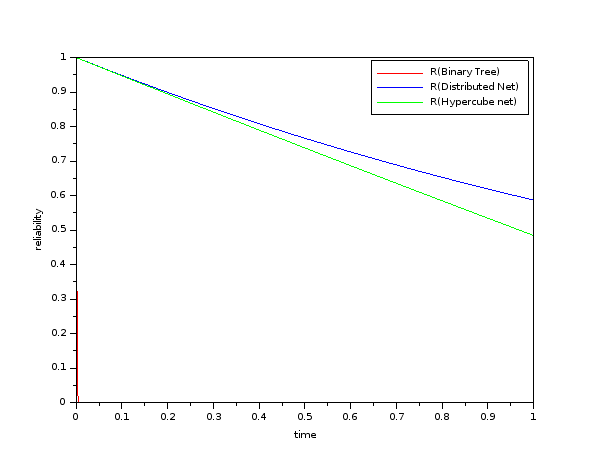
\includegraphics[scale=0.3]{images/comparative_reliablities.png}
		\end{column}
	\end{columns}
\end{frame}